\begin{section}
    {List, Stack, Queue}


\subsection*{1. List}

\subsubsection*{Definition}
A finite, \textbf{ordered} collection of elements. n. length (size) of the List

\bigskip\noindent
List Operations: Insert(x, p, L), Delete(p, L), Next(p, L), Previous(p, L), Locate(p, L), Retrieve(p, L), MakeNull(L), First(L)

\subsubsection*{Array-based list}

\begin{center}
    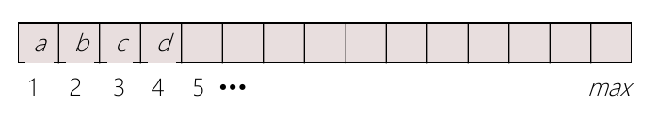
\includegraphics[]{img/arraybasedlist.png}
\end{center}
This, size n = 4
\bigskip
If execute Insert(x, 2, L), then b, c, d will be moved to the right side, then arr[index = 2] will be $x$.

\textbf{TIME COMPLEXITY} :
\begin{tabular}{ccc}
    \textbf{Insert(x, p, L)} : $O(n)$ & \textbf{Delete(p, L)} : $O(n)$ & \textbf{Locate(p, L)} : $O(1)$
\end{tabular}

\subsubsection*{Pointer-based list}

\begin{center}
    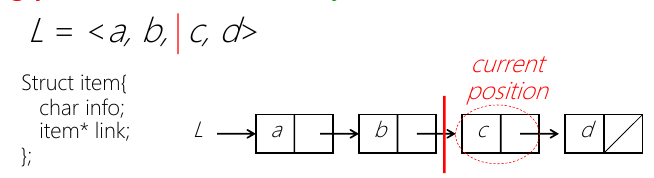
\includegraphics[]{img/pointerbasedlist.png}
\end{center}

\noindent
\textbf{- Singly-linked(one-way)} : each node has a pointer to the next node, and value.

\begin{enumerate}
    \item $P$ direcctly points to the current element.
    Difficulty for insert : hard to access to the preceding node of the current one, but we have to change the link of the preceding node. -> we need a pointer to the preceding node.
    \item \textbf{One-step ahead convention} : $P$ points to the previous element of the current position. $P$ is the position of the preceding node. \\
    When executing Insert(x, p, L) and the list is empty or the left node is empty, we can't use. Solution : add a dummy node at the beginning of the list.
\end{enumerate}

If you know the location(pointer) of the preceding node, then you can insert the new node in $O(1)$ time. But if you don't know, the time complexity is $O(n)$.

\bigskip\noindent
\textbf{- Doubly-linked(two-way)} : each node has a pointer to the next node, and the previous node, and value.
\textbf{Q}. what is the difference between singly-linked and doubly-linked?
\textbf{Solution}: In singly-linked, we can't access to the preceding node of the current one, but in doubly-linked, we can access to the preceding node of the current one. So we can get the previous node of the current one in $O(1)$ time.

The Comparison of singly-linked and doubly-linked is below.
\begin{center}
\begin{tabular}{|c|c|c|c|}
    \hline
    & \textbf{Singly-linked} & \textbf{Doubly-linked} \\
    \hline
    \textbf{Insert(x, p, L)} & $O(n)$ & $O(n)$ \\
    \hline
    \textbf{Delete(p, L)} & $O(n)$ & $O(n)$ \\
    \hline
    \textbf{Locate(p, L)} & $O(n)$ & $O(n)$ \\
    \hline
\end{tabular}
\end{center}

It is similar to the singly-linked list, but we can access to the preceding node of the current one. So we can get the previous node of the current one in $O(1)$ time.

\subsubsection*{Cursor-based list}

\begin{wrapfigure}{r}{3.1cm}
    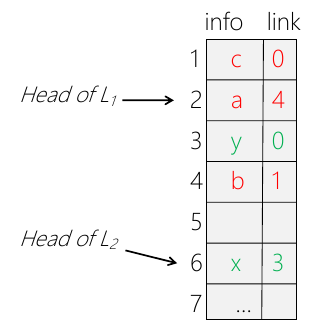
\includegraphics[width=3cm]{img/cursorbasedlist.png}
\end{wrapfigure}

\bigskip
Cursor : simulated pointer. Interger index indicating positions in array to simulate pointers. \\
\textbf{TIME COMPLEXITY} : insert(x, p, L) : $O(1)$, delete(p, L) : $O(1)$, retrieve(p, L) : $O(n)$

\bigskip

\subsection*{2. Stack}

\subsection*{Definition}

All insertion \& deletions take place at one end(Top). LIFO(Last In First Out) structure. You can implement stacks using any type of list implementation(pointer, array, cursor, ...).
\medskip
\noindent Stack Operations: Push(x, S), Pop(S), Top(S), MakeNull(S), IsEmpty(S)

\subsubsection*{Array-based Stack}
How to implement TOP? (in terms of cost of pop/push) \\
Position k(when k elements in stack): $O(1)$ \\ (Fixed) Position 1: $O(n)$

\subsubsection*{Linked stack}

\begin{wrapfigure}{c}{5.1cm}
    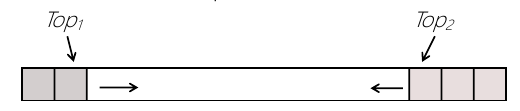
\includegraphics[width=5cm]{img/linkedstack.png}
\end{wrapfigure}

Very much similar to the pointer-based list implementation


\subsection*{3. Queue}

\subsubsection*{Definition}

FIFO(First In First Out) structure. \\
Similar to top in the stack, here we have front and rear
\medskip
\noindent Queue Operations: Enqueue(x, Q), Dequeue(Q), Front(Q), MakeNull(Q), IsEmpty(Q)

\subsubsection*{Array-based Queue}
\begin{itemize}
    \item Simple array implementation \\ "drifting queue" problem. we can solve in an inefficient way. Enqueue \& dequeue : $O(1)$ \& $O(n)$ or vice versa.

    \item \textbf{Circular Queue} 
    \begin{center}
        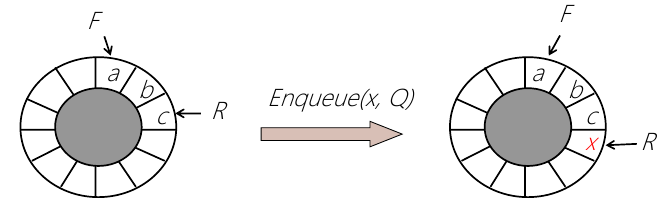
\includegraphics[scale = 0.7]{img/arraybasedqueue.png}
    \end{center}
    Modulus / Modulo operator : Methematically connect the last element to the first element via modulo operator. \\
    Then, we have a problem. How to recognize empty queue or full queue?\\
    Sol 1. Explicit count variable such as cnt. \\ Sol 2. Boolearn variable `isEmpty'
\end{itemize}

\subsubsection*{Linked Queue}
\begin{itemize}
    \item without dummy header,
    Two pointers : (F, R) Empty(Q) is true if F = R = NULL. \\ Enqueue(x, Q) also can, but Problem: Can we use the same code when inserting into an empty queue?
    \item with dummy header,
    Empty(Q) is true if F = R = header.
\end{itemize}

Comparison with header and without header.
Speed? Space utilization? Code conciseness? - insertion into an empty queue, deleteion when queue has only one.

\subsubsection*{Others}

There are other types of queues: queue, circular queue, priority queue, double-ended queue(deque), ...

\bigskip
\end{section}
